\begin{tikzpicture}[>=stealth', node distance=\layersep cm, shorten >=1pt]


        \def\layersep{2}            % vertikal distance between the layers
        \def\neuronsep{1.5}         % Horizontal distance between neurons
        \def\dlsize{1.5}            % distance between node and layer lable
        \def\inout{\layersep*.65}   % Size of in- and output-arrow
        \def\siz{.8}                % neuronsize
        \def\y{3}                   % Start of the most upper layer
        \def\ni{3}                  % Amount of input neurons
        \def\no{2}                  % Amount of output neurons
        \tikzstyle{neuron}=[circle,draw=black,minimum size=\siz cm,inner sep=2pt]
        \tikzstyle{annot} = [text width=5em, text centered]
        \tikzset{fontscale/.style = {font={\fontsize{#1pt}{#1pt}\selectfont}}}
        \tikzset{
                ident/.pic={
                \draw[semithick] (-\siz/#1,-\siz/#1) -- (\siz/#1,\siz/#1);
        }}


        \newcommand{\neurono}[2][]{
            \node[neuron,circle split,inner sep=2pt] (#1) at (#2)
                    {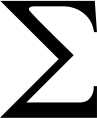
\includegraphics[width=0.225cm]{Bilder/Sigma.png} \nodepart{lower} };
            \pic at ($(#1.lower)-(0,\siz/8)$) {ident=5};
        }
        
        

        % Draw the left input layer nodes
            \foreach \name / \xn in {1,...,\ni}{
            % This is the same as writing \foreach \name / \y in {1/1,2/2,3/3,4/4}
                \node[neuron] (Il-\name) at (\xn*\neuronsep-\neuronsep,\y) [fontscale=15] {$X_{\xn}$};
                \node[above of=Il-\name, node distance=\inout cm] (Inl-\name) {};
                \draw [->,arrows={-Stealth[length=7pt]},densely dotted] (Inl-\name) edge (Il-\name);
            }
            
            \node[fontscale=15] (Il-dot) at ({(\ni+1)*\neuronsep-\neuronsep},\y) {$\dots$};
            
            \node[neuron,fontscale=15] (Il-i) at ({(\ni+2)*\neuronsep-\neuronsep},\y) {$X_{i}$};
            \node[above of=Il-i, node distance=\inout cm] (Inl-i) {};
            \draw [->,arrows={-Stealth[length=7pt]},densely dotted] (Inl-i) edge (Il-i);
            
            

        % Draw the output layer node
            \foreach \name / \xn in {1,...,\no}{
                \node[neuron] (Ol-\xn) at ({(\ni-1)*\neuronsep/2-\neuronsep/2*(\no-1)+(\xn-1)*\neuronsep},\y-\layersep) [fontscale=15] {$Y_{\xn}$};
                
                \node[node distance=\inout cm, below of=Ol-\xn] (Onl) {};
                
                \draw [->,arrows={-Stealth[length=7pt]},densely dotted] (Ol-\xn) edge (Onl);
            }
            
            \node[fontscale=15] (Ol-dot) at ({(\ni-1)*\neuronsep/2-\neuronsep/2*(\no+1)+(\no+1)*\neuronsep},\y-1*\layersep)  {$\dots$};
                
                \node[neuron,fontscale=15] (Ol-o) at ({(\ni-1)*\neuronsep/2-\neuronsep/2*(\no+2)+(\no+2.5)*\neuronsep},\y-1*\layersep)  {$Y_o$};
                \node[node distance=\inout cm, below of=Ol-o] (Onl) {};
                \draw [->,arrows={-Stealth[length=7pt]},densely dotted] (Ol-o) edge (Onl);  
                
              
        % Connect every node in the input layer with the output layer
            \foreach \name / \xn in {1,...,\no,o}{
            \foreach \source in {1,...,\ni,i}
                \draw [->,arrows={-Stealth[length=7pt]}] (Il-\source) edge (Ol-\xn);
            }
                
                
        % Annotate the layers
                \node[annot,right of=Il-i, node distance=\dlsize cm] (il) {\textbf{Eingabe- schicht}};
                \node[annot,below of=il] {\textbf{Ausgabe- schicht}};
        %-----------------------------------------
        %% rechtes Bild

        % Draw the right input layer nodes
                \node[xshift=\dlsize cm] (Ir) at (il) {};
            \foreach \name / \xn in {1,...,\ni}{
        % This is the same as writing \foreach \name / \y in {1/1,2/2,3/3,4/4}
                \node[neuron] (Ir-\name) at ($(Ir)+(\xn*\neuronsep-\neuronsep,0)$) {};
                \node[above of=Ir-\name, node distance=\inout cm] (Inr-\name) {};
                \pic at (Ir-\name) {ident=4};
                \draw [->,arrows={-Stealth[length=7pt]},densely dotted] (Inr-\name) edge (Ir-\name);
            }
            
            \node[fontscale=15] (Ir-dot) at ($(Ir)+({(\ni+1)*\neuronsep-\neuronsep},0)$) {$\dots$};
            
            \node[neuron,fontscale=15] (Ir-i) at ($(Ir)+({(\ni+2)*\neuronsep-\neuronsep},0)$) {};
            \pic at (Ir-i) {ident=4};
            \node[above of=Ir-i, node distance=\inout cm] (Inr-i) {};
            \draw [->,arrows={-Stealth[length=7pt]},densely dotted] (Inr-i) edge (Ir-i);
            
        % Draw the output layer node
            \foreach \name / \xn in {1,...,\no}{
                \neurono[Or-\xn]{$(Ir)+({(\ni-1)*\neuronsep/2-\neuronsep/2*(\no-1)+(\xn-1)*\neuronsep},-\layersep)$}

                \node[node distance=\inout cm, below of=Or-\xn] (Onr) {};
                
                \draw [->,arrows={-Stealth[length=7pt]},densely dotted] (Or-\xn) edge (Onr);
            }
            
             \node[fontscale=15] (Or-dot) at ($(Ir)+({(\ni-1)*\neuronsep/2-\neuronsep/2*(\no+1)+(\no+1)*\neuronsep},-\layersep)$)  {$\dots$};
                
                \neurono[Or-o]{$(Ir)+({(\ni-1)*\neuronsep/2-\neuronsep/2*(\no+2)+(\no+2.5)*\neuronsep},-\layersep)$}
                \node[node distance=\inout cm, below of=Or-o] (Onr) {};
                \draw [->,arrows={-Stealth[length=7pt]},densely dotted] (Or-o) edge (Onr);    
                
        % Connect every node in the input layer with the output layer
            \foreach \name / \xn in {1,...,\no,o}{
            \foreach \source in {1,...,\ni,i}
                \draw [->,arrows={-Stealth[length=7pt]},every node/.style={fill=white,inner sep=1pt,fontscale=7}] 
                (Ir-\source) edge  (Or-\xn);
            }
        
            \draw [fill=white,draw=black, dotted] ($(Ir-1)+(\neuronsep/4-.45,-\layersep*.6)$) rectangle ($(Ir-i)+(\neuronsep/100,-\layersep*.375)$);
                
            \node[fill=white,inner sep=1pt,fontscale=10] at ($(Ir-1)+({(\ni+1)*\neuronsep/2},-\layersep*.5)$) {$\dots\,w_{o,i}\,\dots$};
        
        \end{tikzpicture}